\documentclass[11pt,a4paper,oneside]{article}
\usepackage[a4paper,margin=27mm,headheight=22pt]{geometry}
\usepackage[T1]{fontenc}
\usepackage{newtxtext,newtxmath}
\usepackage{microtype}
\usepackage{amsmath,mathtools,bm}
\usepackage{graphicx}
\usepackage{booktabs,tabularx,array}
\usepackage{caption,subcaption}
\usepackage{xcolor}
\usepackage{titlesec}
\usepackage{fancyhdr}
\usepackage{enumitem}
\usepackage{listings}
\usepackage[most]{tcolorbox}
\usepackage{hyperref}
\usepackage[nameinlink,noabbrev]{cleveref}
\usepackage{setspace}
\usepackage{float}
\usepackage{needspace}
\definecolor{ink}{HTML}{1E293B}
\definecolor{muted}{HTML}{64748B}
\definecolor{accent}{HTML}{245B78}
\definecolor{pale}{HTML}{F3F6F8}
\definecolor{rule}{HTML}{D8E1E8}
\hypersetup{colorlinks=true,linkcolor=accent,citecolor=accent,urlcolor=accent,pdftitle={Brownian Motion and Measure Theory},pdfauthor={Yasin Saifi},pdfsubject={Student-Selected Independent Study Project; Final Project for Stochastic Processes}}
\setstretch{1.12}
\setlength{\parindent}{0pt}
\setlength{\parskip}{5pt plus 1pt}
\setlist[itemize]{leftmargin=1.6em,itemsep=2pt,topsep=3pt}
\setlist[enumerate]{leftmargin=1.8em,itemsep=3pt,topsep=3pt}
\titleformat{\section}{\Large\bfseries\color{ink}}{\thesection}{0.7em}{}
\titleformat{\subsection}{\large\bfseries\color{accent}}{\thesubsection}{0.7em}{}
\titlespacing*{\section}{0pt}{22pt}{9pt}
\titlespacing*{\subsection}{0pt}{13pt}{5pt}
\pagestyle{fancy}
\fancyhf{}
\fancyhead[L]{\small\color{muted}Brownian Motion and Measure Theory}
\fancyhead[R]{\small\color{muted}\nouppercase{\rightmark}}
\fancyfoot[C]{\small\color{muted}\thepage}
\renewcommand{\headrulewidth}{0.4pt}
\renewcommand{\headrule}{\hbox to\headwidth{\color{rule}\leaders\hrule height \headrulewidth\hfill}}
\captionsetup{font=small,labelfont=bf,skip=6pt}
\lstdefinestyle{python}{language=Python,basicstyle=\ttfamily\small,keywordstyle=\bfseries\color{accent},commentstyle=\itshape\color{muted},stringstyle=\color{ink},showstringspaces=false,frame=single,rulecolor=\color{rule},backgroundcolor=\color{pale},breaklines=true,columns=fullflexible,keepspaces=true,xleftmargin=5pt,xrightmargin=5pt,aboveskip=7pt,belowskip=8pt}
\newtcolorbox{keyidea}{colback=pale,colframe=rule,boxrule=.5pt,arc=2mm,left=3mm,right=3mm,top=2mm,bottom=2mm}
\newcommand{\E}{\mathbb{E}}
\newcommand{\Prob}{\mathbb{P}}
\newcommand{\R}{\mathbb{R}}
\newcommand{\Borel}{\mathcal{B}}
\newcommand{\F}{\mathcal{F}}
\newcommand{\Om}{\Omega}
\newcommand{\dd}{\,\mathrm{d}}
\newcommand{\Var}{\operatorname{Var}}
\newcommand{\Law}{\mathcal{L}}
\newcommand{\ind}{\mathbf{1}}

\begin{document}
\hypersetup{pageanchor=false}
\begin{titlepage}
\thispagestyle{empty}
\vspace*{10mm}
{\color{accent}\rule{\textwidth}{1.2pt}}\\[8mm]
{\Huge\bfseries\color{ink} Brownian Motion\\[2mm] and Measure Theory}\\[4mm]
{\Large\color{muted} A student-selected independent study project}\\[3mm]
{\large\color{muted} Final Project for the Course Stochastic Processes}\\[8mm]
{\color{accent}\rule{0.34\textwidth}{1.2pt}}\\[7mm]
\begin{keyidea}
This student-selected independent study project was undertaken as the final project for the course Stochastic Processes, with the instructor's approval. It provides a structured study of selected topics extending the foundational course material, with the aim of developing a clear mathematical understanding and preparing the material for classroom presentation and discussion.
\end{keyidea}
\vspace{4mm}
\begin{center}
\begin{tabular}{@{}rl@{}}
\textcolor{muted}{Course:} & Stochastic Processes \\[2mm]
\textcolor{muted}{Instructor:} & Dr. Hossein Peyvandi \\[2mm]
\textcolor{muted}{Prepared by:} & Yasin Saifi
\end{tabular}
\end{center}
\vfill
\begin{center}
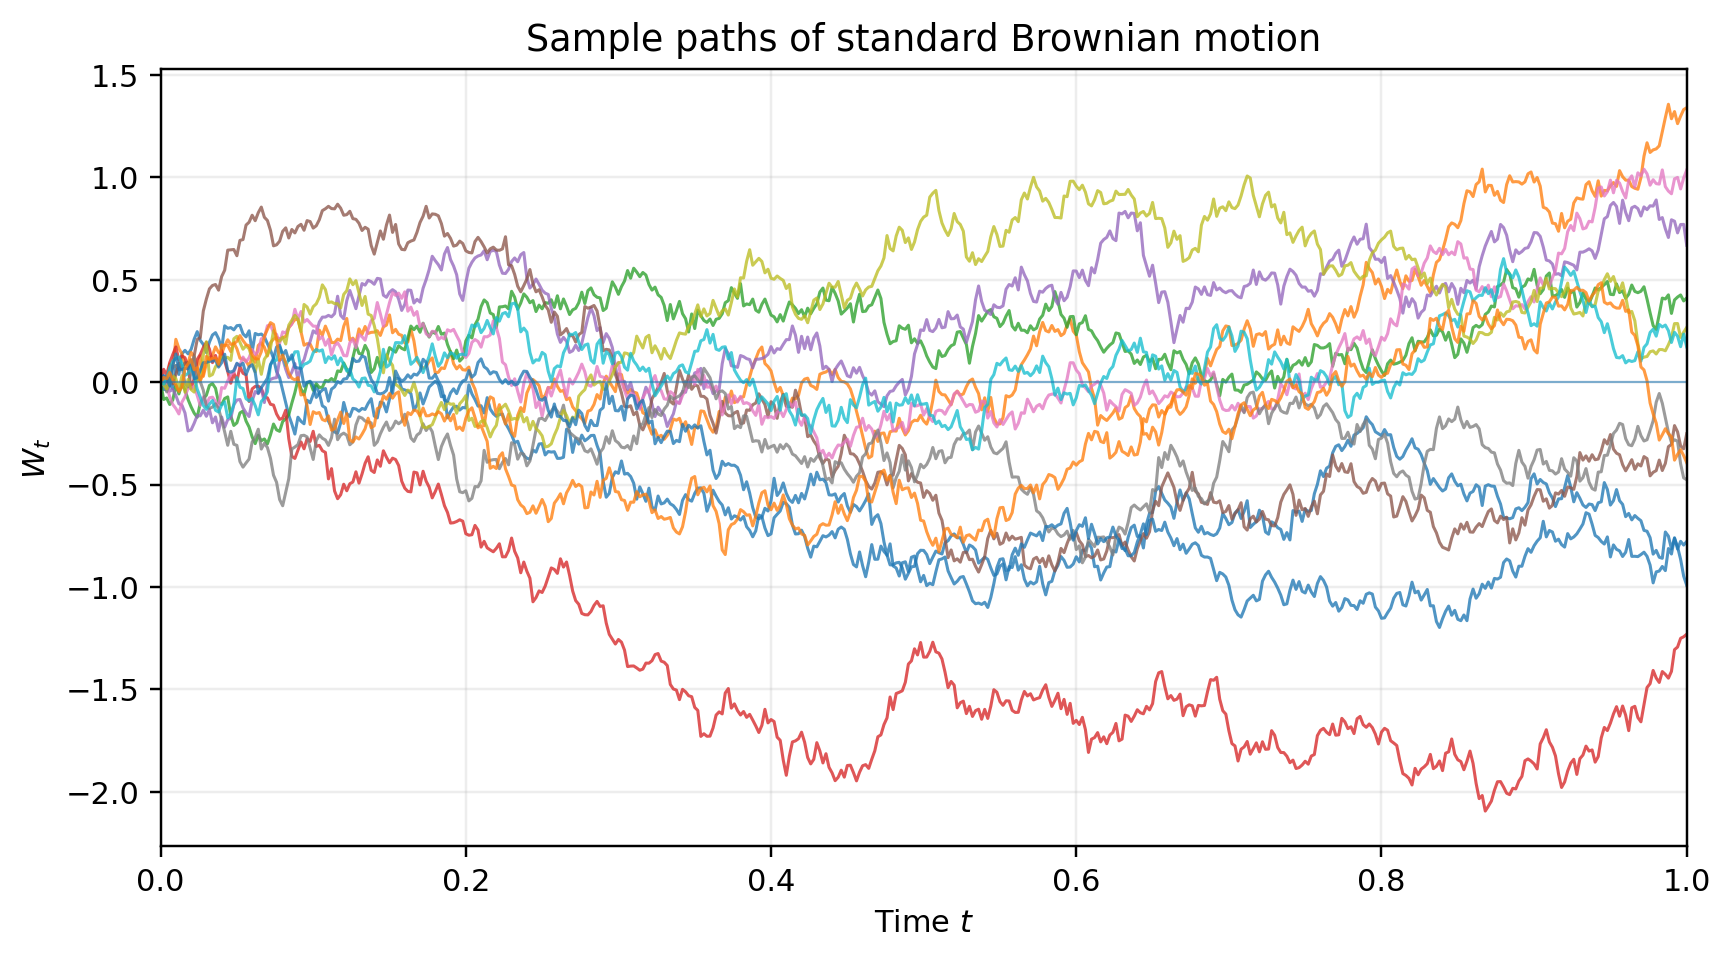
\includegraphics[width=0.82\textwidth]{figures/01_brownian_paths.png}\\[2mm]
{\small\color{muted}Simulated sample paths of standard Brownian motion on $[0,1]$.}
\end{center}
\vfill
{\small\color{muted}Mathematical exposition $\mid$ Python simulations $\mid$ Reproducibility}
\end{titlepage}

\pagenumbering{roman}
\section*{Abstract}
This report presents a student-selected independent study project undertaken as the final project for the course Stochastic Processes, with the instructor's approval. The topic was selected to provide an opportunity for focused study of measure-theoretic probability and standard Brownian motion, and to develop material suitable for presentation and discussion in class. The mathematical exposition covers measurable spaces, sigma-algebras, probability measures, measurable random variables, probability distributions, expectation as a Lebesgue integral, and the defining properties of standard Brownian motion. The computational component illustrates Gaussian increments, sample paths, quadratic variation along increasingly fine partitions, and an ordinary time integral of a Brownian path.

The presentation combines definitions, mathematical derivations, and numerical experiments. Each computational illustration is accompanied by the relevant theoretical relationship, allowing the simulated results to be interpreted in the context of the mathematical development.

\setcounter{tocdepth}{1}
\tableofcontents
\clearpage
\hypersetup{pageanchor=true}
\pagenumbering{arabic}

\section{Measure-theoretic foundations}
\subsection{Sample spaces and events}
A sample space $\Om$ is the set of possible outcomes of a random experiment. An event is a subset of $\Om$. To assign probabilities consistently, a collection of events closed under the set operations required in probability theory is specified.

\subsection{Sigma-algebras and measurable spaces}
A \emph{sigma-algebra} $\F$ on $\Om$ is a collection of subsets of $\Om$ satisfying:
\begin{enumerate}
  \item $\Om\in\F$;
  \item if $A\in\F$, then $A^c\in\F$;
  \item if $A_1,A_2,\ldots\in\F$, then $\displaystyle\bigcup_{n=1}^{\infty}A_n\in\F$.
\end{enumerate}
The pair $(\Om,\F)$ is called a \emph{measurable space}. The requirement of closure under countable unions is important when events are defined through limits. On the real line, the standard measurable structure is the Borel sigma-algebra $\Borel(\R)$, generated by open subsets of $\R$.

\subsection{Measures and probability measures}
A measure $\mu$ assigns a nonnegative value to each measurable set, satisfies $\mu(\varnothing)=0$, and is countably additive over pairwise disjoint sets. A probability measure is a measure $\Prob$ with total mass one:
\begin{equation}\label{eq:countadd}
 \Prob\!\left(\bigcup_{n=1}^{\infty}A_n\right)
 =\sum_{n=1}^{\infty}\Prob(A_n),
 \qquad \text{if the }A_n\text{ are pairwise disjoint},
\end{equation}
and $\Prob(\Om)=1$. A probability space is a triple $(\Om,\F,\Prob)$.

\begin{keyidea}
The measure-theoretic viewpoint separates three ingredients: the outcomes ($\Om$), the events to which probabilities may be assigned ($\F$), and the rule assigning probabilities ($\Prob$). This structure is the starting point for defining Brownian motion rigorously.
\end{keyidea}

\subsection{Why this framework is useful}
Countable additivity implies useful continuity properties. For example, if $A_n\uparrow A$, then $\Prob(A_n)\uparrow\Prob(A)$. Such results justify passing from finite approximations to limiting events. Similar limit ideas appear when studying increasingly fine time partitions of a stochastic process.

\section{Random variables, distributions, and expectation}
\subsection{Measurable random variables}
A real-valued random variable is a measurable map
\[
 X:(\Om,\F)\longrightarrow(\R,\Borel(\R)).
\]
Measurability means that $X^{-1}(B)=\{\omega\in\Om:X(\omega)\in B\}$ belongs to $\F$ for every Borel set $B$. This condition guarantees that events defined in terms of $X$ have well-defined probabilities.

\subsection{The law of a random variable}
The distribution, or law, of $X$ is the probability measure on $\R$ defined by
\begin{equation}\label{eq:law}
 \Law(X)(B)=\Prob(X\in B)=\Prob\bigl(X^{-1}(B)\bigr),
 \qquad B\in\Borel(\R).
\end{equation}
Thus, a random variable is a measurable function on the original sample space, whereas its law is a probability measure on the real line. The law records the probabilities of ranges of values without requiring the underlying outcome $\omega$.

\subsection{Expectation as a Lebesgue integral}
For a simple random variable $X=\sum_{j=1}^{m}a_j\ind_{A_j}$, where the sets $A_j$ are disjoint and measurable, define
\[
 \E[X]=\sum_{j=1}^{m}a_j\Prob(A_j).
\]
A nonnegative measurable random variable can be approximated from below by simple random variables. Taking the corresponding limit gives the Lebesgue integral. For an integrable random variable,
\begin{equation}\label{eq:expect}
 \E[X]=\int_{\Om}X(\omega)\,\dd\Prob(\omega).
\end{equation}
The Lebesgue integral is the natural definition of expectation in measure-theoretic probability. In computations, sample averages are used to approximate expectations, while the mathematical definition remains the integral in \cref{eq:expect}.

\subsection{Variance and modes of convergence}
For a square-integrable random variable,
\[
 \Var(X)=\E\bigl[(X-\E[X])^2\bigr].
\]
Two useful notions of convergence are:
\begin{itemize}
 \item $X_n\to X$ in probability if $\Prob(|X_n-X|>\varepsilon)\to0$ for every $\varepsilon>0$;
 \item $X_n\to X$ almost surely if $\Prob(\{\omega:X_n(\omega)\to X(\omega)\})=1$.
\end{itemize}
The distinction matters: some simulation results concern averages over many paths, while theoretical statements about quadratic variation are formulated as convergence of random variables.

\section{Standard Brownian motion}
\subsection{Definition}
A standard Brownian motion is a stochastic process $W=(W_t)_{t\geq0}$ satisfying the following properties:
\begin{enumerate}
 \item $W_0=0$ almost surely;
 \item the sample paths $t\mapsto W_t$ are continuous almost surely;
 \item it has independent increments;
 \item for $0\leq s<t$, the increment is Gaussian with mean zero and variance $t-s$:
 \begin{equation}\label{eq:increment}
   W_t-W_s\sim N(0,t-s).
 \end{equation}
\end{enumerate}
The final property is often called the Gaussian increment property. Together with independent increments, it determines the finite-dimensional distributions of standard Brownian motion.

\subsection{Consequences of the definition}
Setting $s=0$ in \cref{eq:increment} gives
\begin{equation}\label{eq:marginal}
 W_t\sim N(0,t),\qquad \E[W_t]=0,\qquad \Var(W_t)=t.
\end{equation}
The variance grows linearly with time. Also, the distribution of an increment depends only on the length of the interval, not on its starting point. Hence Brownian motion has stationary increments in distribution.

For $0\leq s\leq t$, write $W_t=W_s+(W_t-W_s)$. Since the increment is independent of $W_s$ and has mean zero,
\begin{align}\label{eq:covariance}
 \operatorname{Cov}(W_s,W_t)
 &=\E[W_sW_t]-\E[W_s]\E[W_t]\\
 &=\E[W_s^2]=s.
\end{align}
Consequently, for all $s,t\geq0$,
\[
 \operatorname{Cov}(W_s,W_t)=\min(s,t).
\]

\subsection{A note on simulated paths}
A computer stores finitely many values of a process. In the figures, values are simulated at grid points and joined by straight line segments. The displayed polyline is a visualization of the sampled values; it is not an exact rendering of the continuous Brownian path between grid points.
\begin{figure}[H]
 \centering
 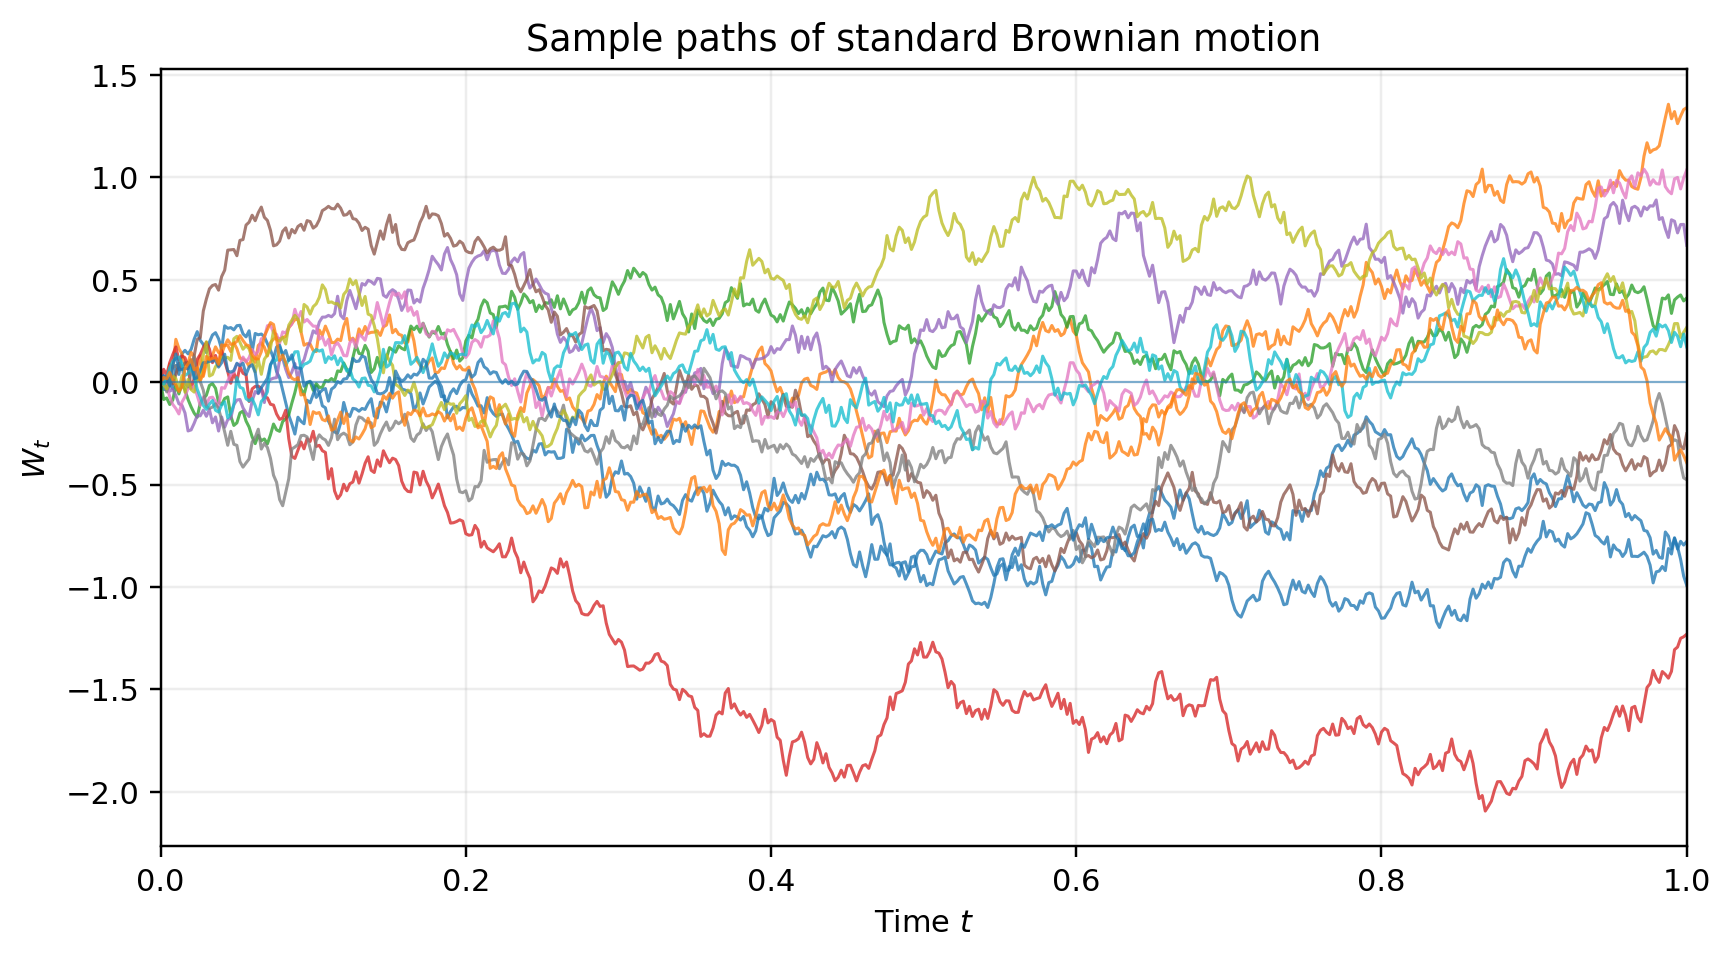
\includegraphics[width=0.93\textwidth]{figures/01_brownian_paths.png}
 \caption{Twelve simulated Brownian paths on $[0,1]$, using 500 equal time intervals per path.}
 \label{fig:paths}
\end{figure}

\section{Simulation method}
\subsection{Constructing the increments}
Fix a time horizon $T>0$ and an integer $n\geq1$. Use the equally spaced grid
\[
 0=t_0<t_1<\cdots<t_n=T,
 \qquad \Delta t=\frac{T}{n}.
\]
Let $Z_0,\ldots,Z_{n-1}$ be independent standard normal random variables. Define
\begin{equation}\label{eq:sim}
 \Delta W_k=\sqrt{\Delta t}\,Z_k,
 \qquad
 W_{t_k}=\sum_{j=0}^{k-1}\Delta W_j,
 \quad k=1,\ldots,n.
\end{equation}
Then the increments are independent and satisfy $\Delta W_k\sim N(0,\Delta t)$, precisely as required by \cref{eq:increment}. Therefore the generated values reproduce the finite-dimensional distribution of standard Brownian motion on the chosen grid.

\clearpage
\subsection{Implementation}
The core implementation uses NumPy's random number generator. The array is organized so that each column represents one simulated path and each row represents one time point.
\begin{lstlisting}[style=python,caption={Simulation of standard Brownian motion on an equally spaced grid.},label={lst:simulation}]
def simulate_brownian(T=1.0, n_steps=500,
                      n_paths=20, seed=2026):
    rng = np.random.default_rng(seed)
    dt = T / n_steps
    dW = np.sqrt(dt) * rng.standard_normal(
        (n_steps, n_paths)
    )
    paths = np.vstack((
        np.zeros((1, n_paths)),
        np.cumsum(dW, axis=0)
    ))
    times = np.linspace(0.0, T, n_steps + 1)
    return times, paths
\end{lstlisting}
The factor $\sqrt{\Delta t}$ is essential: if $Z_k\sim N(0,1)$, then $\sqrt{\Delta t}Z_k\sim N(0,\Delta t)$. A fixed seed makes the numerical output reproducible; changing the seed produces a different realization without changing the target distribution.

\section{Numerical experiments}
\subsection{Experiment 1: distribution of increments}
For a Brownian increment over an interval of length $\Delta t$, the theoretical density is
\[
 f_{\Delta W}(x)=\frac{1}{\sqrt{2\pi\Delta t}}
 \exp\!\left(-\frac{x^2}{2\Delta t}\right),
 \qquad x\in\R.
\]
The histograms below compare simulated increments with this density for two grid resolutions. As the interval becomes shorter, both the variance and the typical magnitude of the increment decrease.
\begin{figure}[H]
 \centering
 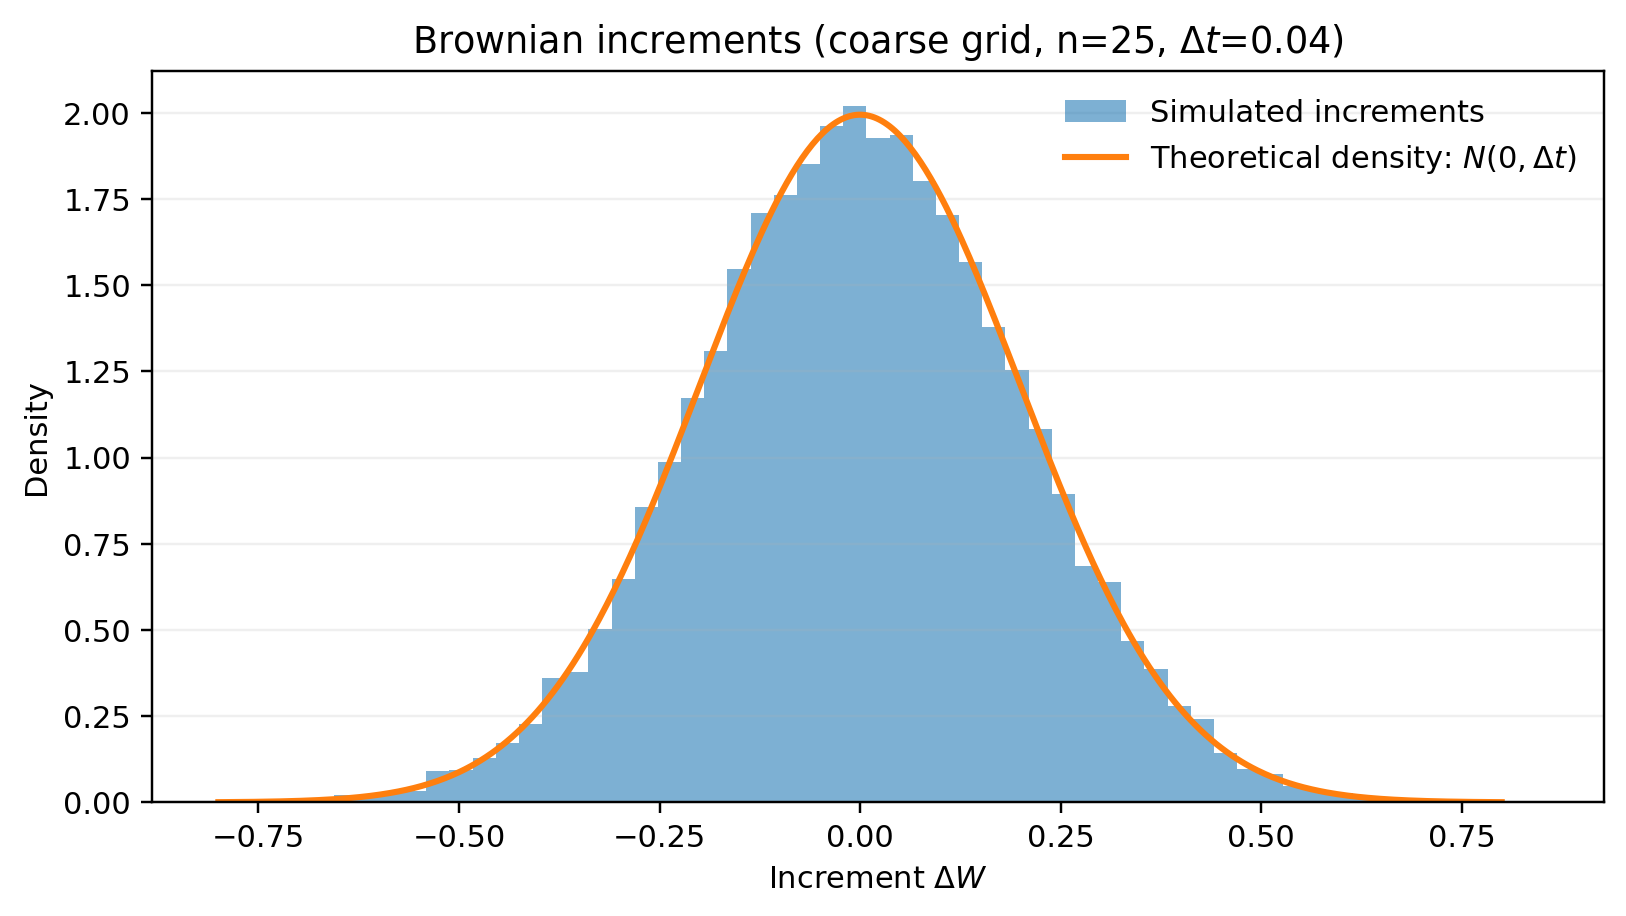
\includegraphics[width=0.88\textwidth]{figures/02_increment_coarse.png}
 \caption{Increment distribution for a coarse grid with $n=25$ and $\Delta t=0.04$.}
 \label{fig:coarseincrements}
\end{figure}
\begin{figure}[H]
 \centering
 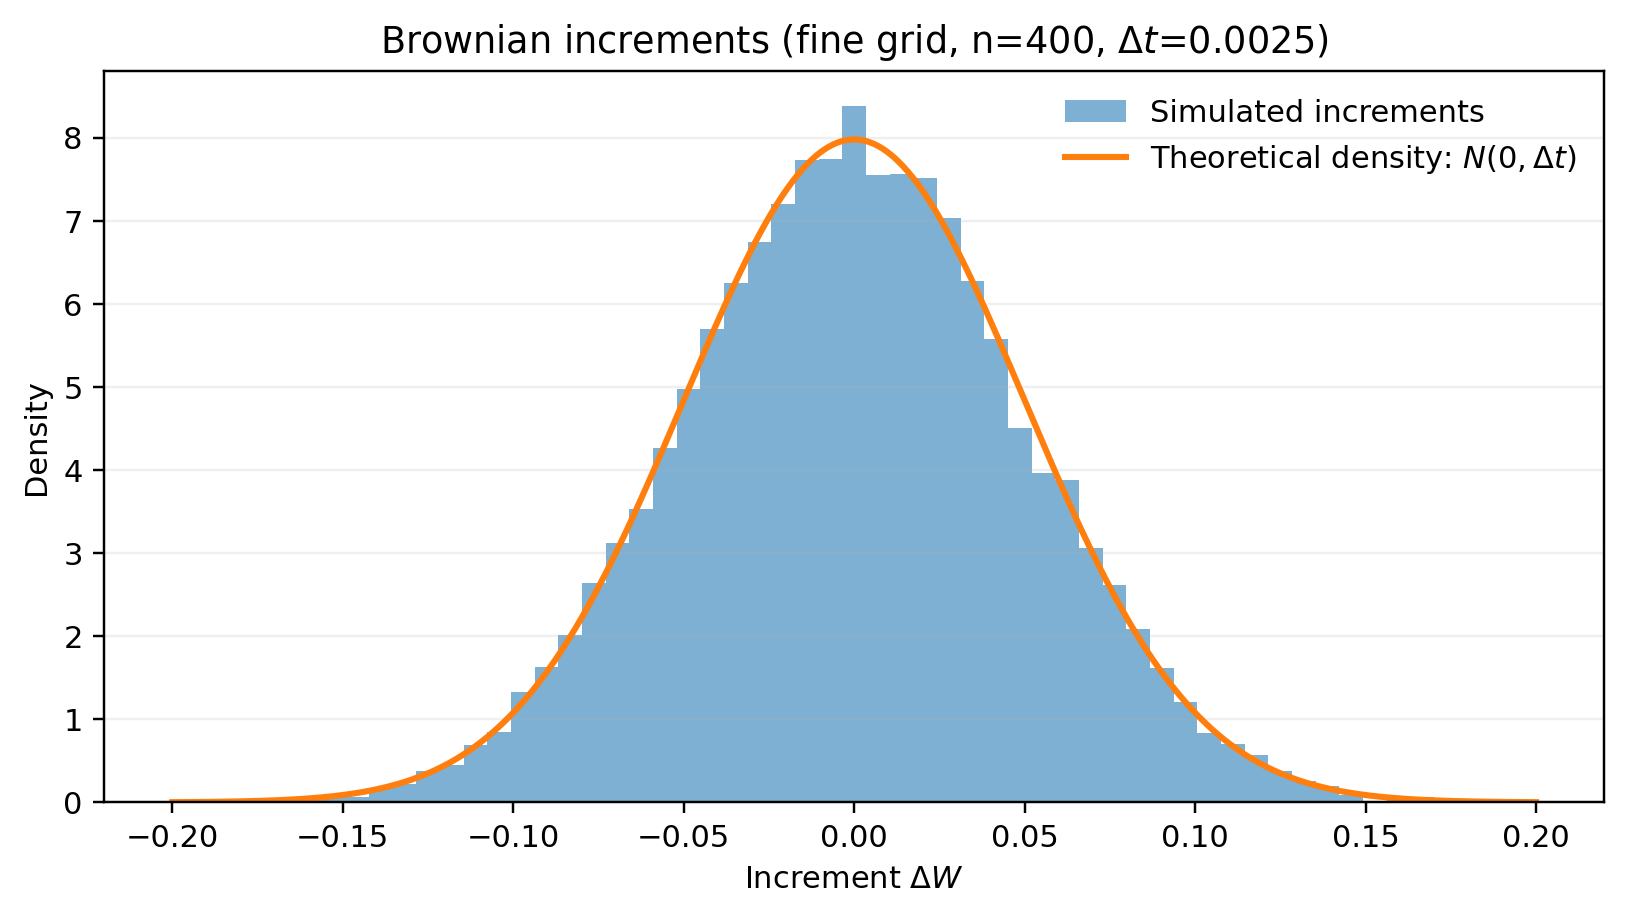
\includegraphics[width=0.88\textwidth]{figures/02_increment_fine.png}
 \caption{Increment distribution for a fine grid with $n=400$ and $\Delta t=0.0025$.}
 \label{fig:fineincrements}
\end{figure}

\clearpage
\subsection{Experiment 2: quadratic variation}
For an equal partition of $[0,T]$, define the discrete quadratic variation
\begin{equation}\label{eq:qv}
 Q_n=\sum_{k=0}^{n-1}(W_{t_{k+1}}-W_{t_k})^2.
\end{equation}
Since each increment is distributed as $N(0,\Delta t)$, its squared value has expectation $\Delta t$ and variance $2(\Delta t)^2$. This follows from $\E[Z^2]=1$ and $\E[Z^4]=3$ for a standard normal random variable $Z$. Independence of the increments therefore gives
\begin{equation}\label{eq:qvmoments}
 \E[Q_n]=T,
 \qquad
 \operatorname{Var}(Q_n)=2n(\Delta t)^2=\frac{2T^2}{n}.
\end{equation}
It follows that
\[
 \E[(Q_n-T)^2]=\frac{2T^2}{n}\longrightarrow0.
\]
Thus $Q_n\to T$ in mean square, and consequently in probability. The simulation below compares the empirical mean and cross-path standard deviation of $Q_n$ with the theoretical behavior. The error bars show one standard deviation across simulated paths; they are not confidence intervals for the mean.
\begin{figure}[H]
 \centering
 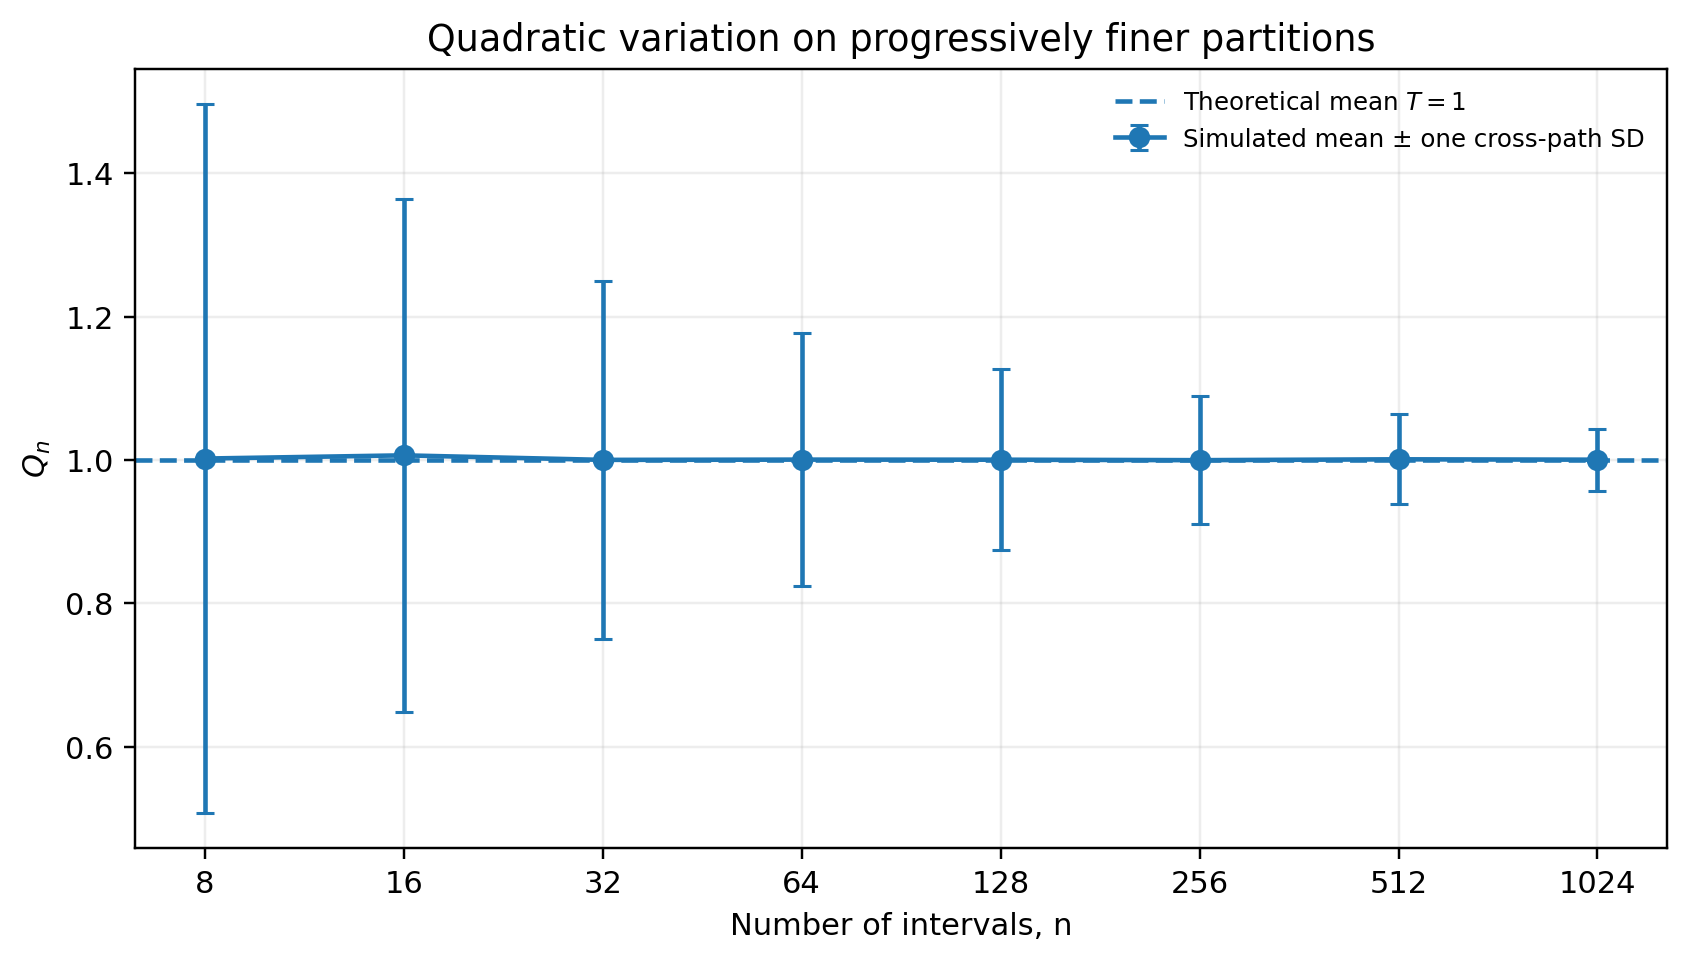
\includegraphics[width=0.9\textwidth]{figures/03_quadratic_variation.png}
 \caption{Discrete quadratic variation for increasingly fine partitions. The dashed line marks the theoretical mean $T=1$. Error bars show one cross-path standard deviation.}
 \label{fig:qv}
\end{figure}

\Needspace{15\baselineskip}
\subsection{Experiment 3: an ordinary time integral}
Consider the ordinary time integral
\begin{equation}\label{eq:itime}
 I_T=\int_0^T W_t\,\dd t.
\end{equation}
This is the ordinary time integral of a Brownian sample path. It can be approximated by the left-endpoint Riemann sum
\[
 I_T^{(n)}=\Delta t\sum_{k=0}^{n-1}W_{t_k}.
\]
The process is centered, so $\E[I_T]=0$. Its variance can be computed from the covariance function:
\begin{align*}
 \Var(I_T)
 &=\int_0^T\int_0^T\operatorname{Cov}(W_s,W_t)\,\dd s\,\dd t\\
 &=\int_0^T\int_0^T\min(s,t)\,\dd s\,\dd t
 =\frac{T^3}{3}.
\end{align*}
Since Brownian motion is a Gaussian process, this time integral is normally distributed:
\begin{equation}\label{eq:itime-law}
 I_T\sim N\!\left(0,\frac{T^3}{3}\right).
\end{equation}
The histogram below compares simulated Riemann sums with the density in \cref{eq:itime-law} for $T=1$.
\begin{figure}[H]
 \centering
 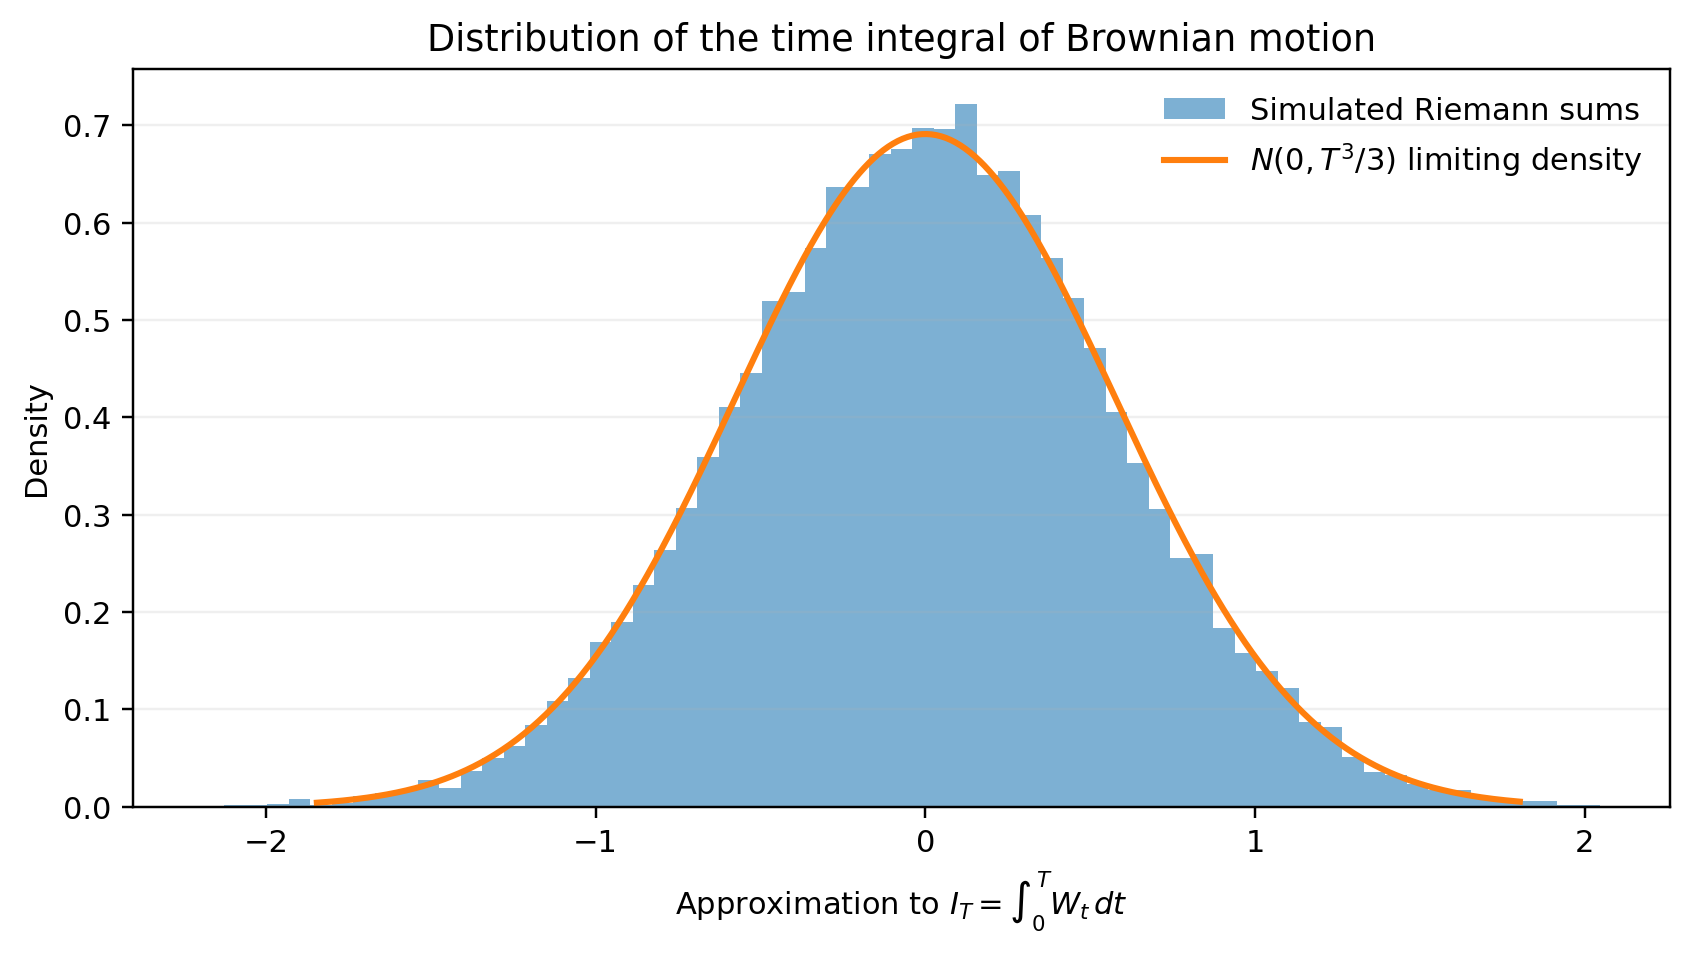
\includegraphics[width=0.9\textwidth]{figures/04_time_integral.png}
 \caption{Distribution of 20,000 simulated left-endpoint Riemann sums, compared with the limiting normal density $N(0,1/3)$.}
 \label{fig:timeintegral}
\end{figure}

\section{Experimental design and reproducibility}
The main experiments use the following settings. The random seeds are fixed so that the figures can be regenerated exactly in the same software environment.
\begin{table}[H]
\centering
\caption{Parameters used in the report's numerical experiments.}
\label{tab:parameters}
\begin{tabularx}{\textwidth}{@{}l X l@{}}
\toprule
Experiment & Main parameters & Seed \\
\midrule
Sample paths & $T=1$, $n=500$, 12 paths & 2026 \\
Increment distributions & 20,000 increments; $n=25$ and $n=400$ & 2052, 2427 \\
Quadratic variation & $n=8,16,\ldots,1024$; 6,000 paths per grid & 2028 \\
Time integral & $T=1$, $n=500$, 20,000 paths & 2029 \\
\bottomrule
\end{tabularx}
\end{table}

To reproduce the experiments, install the packages in \texttt{src/requirements.txt} and execute:
\begin{lstlisting}[style=python]
python -m pip install -r src/requirements.txt
python src/run_experiments.py
\end{lstlisting}
The simulation routines are separated from the plotting script, allowing the Brownian generator to be reused in additional experiments without modification.

\Needspace{13\baselineskip}
\section{Concluding discussion}
The study develops a sequence of ideas connecting the measure-theoretic formulation of probability with the definition and properties of standard Brownian motion. Measurable spaces and probability measures provide the underlying mathematical structure; measurable random variables and their laws describe real-valued quantities on that space; and Lebesgue integration gives a general definition of expectation.

The discussion of Brownian motion brings these ideas together through the properties of Gaussian increments, independence, continuity of sample paths, and the covariance function. The computational experiments provide concrete illustrations of these properties. In particular, the simulations display the behavior of sample paths, the scaling of increment distributions, and the approach of discrete quadratic variation toward the length of the time interval. The calculation of the time integral also demonstrates how the covariance structure of Brownian motion can be used to derive distributional information.

The combination of mathematical exposition and reproducible computational work forms a structured basis for further study and for the presentation of the selected topics in the Stochastic Processes course.

\section*{References}
{\small\setlength{\parskip}{1pt}
\begin{enumerate}[label={[\arabic*]},leftmargin=1.5em,itemsep=1pt,topsep=2pt]
 \item P. Billingsley, \emph{Probability and Measure}, 3rd ed., Wiley, 1995.
 \item D. Stirzaker, \emph{Stochastic Processes and Models}, Oxford University Press, 2005.

\end{enumerate}}

\end{document}
